
\documentclass[ms.tex]{subfiles}
\begin{document}

\section{Nucleosynthesis}
\label{sec:yields}

In this paper we make use of the chemical evolution model for the Milky Way
presented in~\citet{Johnson2021}.
This model runs using the publicly available~\texttt{Versatile Integrator for
Chemical Evolution} (\vice;~\citealp{Johnson2020, Griffith2021, Johnson2021}),
an open-source~\python~package designed for GCE modeling.
\citet{Johnson2021} focus their discussion of the model predictions on O and
Fe, and we retain their yields of these elements here.
As required by~\vice, the SN yields are defined as the net mass of some element
X produced over all explosion events in units of the progenitor cluster's
mass.
For example, with a yield of~$y_\text{X} = 0.001$, a hypothetical~$1000 M_\odot$
star cluster would produce~$1 M_\odot$ of the element X instantaneously in the
case of core collapse supernovae (CCSNe) or over the delay-time distribution
(DTD) in the case of SNe Ia.
We adopt the following values from~\citet{Johnson2021}, who in turn base them
off of~\citet*{Weinberg2017} and~\citet{Johnson2020}:
\begin{itemize}
	\item $\ycc{O} = 0.015$

	\item $\ycc{Fe} = 0.0012$

	\item $\yia{O} = 0$

	\item $\yia{Fe} = 0.00214$
\end{itemize}
We also assume that N is not produced in significant amounts by SNe Ia
\citep{Johnson2019}, and set~$\yia{N} = 0$ throughout this paper
accordingly.
We spend the remainder of this section detailing our CCSN and AGB star yields
of N.

\subsection{Core Collapse Supernovae and Massive Star Winds}
\label{sec:yields:ccsne}

In~\vice, CCSN nucleosynthetic products are approximated to be produced
instantaneously following an episode of star formation; this is a valid
approximation due to how short the lives of massive stars are compared to the
relevant timescales for GCE.
Based on this and its definition as being in units of a stellar population's
total mass, the yield is simply the constant of proportionality between the
CCSN production rate and the star formation rate (SFR):
\begin{equation}
\dot{M}_\text{X}^\text{CC} = \ycc{X}\dot{M}_\star
\end{equation}
More generally,~\ycc{X}~quantifies~\textit{all} of the nucleosynthetic material
approximated to be produced instantaneously following a single stellar
population's formation, though the majority of such events for which this
approximation is valid will be associated with massive stars and/or their
supernovae.
In the case of N specifically, a substantial amount emerges in winds before the
actual supernova itself, allowing massive stars to produce a lot N even if they
collapse directly to a black hole~\citep{Griffith2021}.

\begin{figure*}
\centering
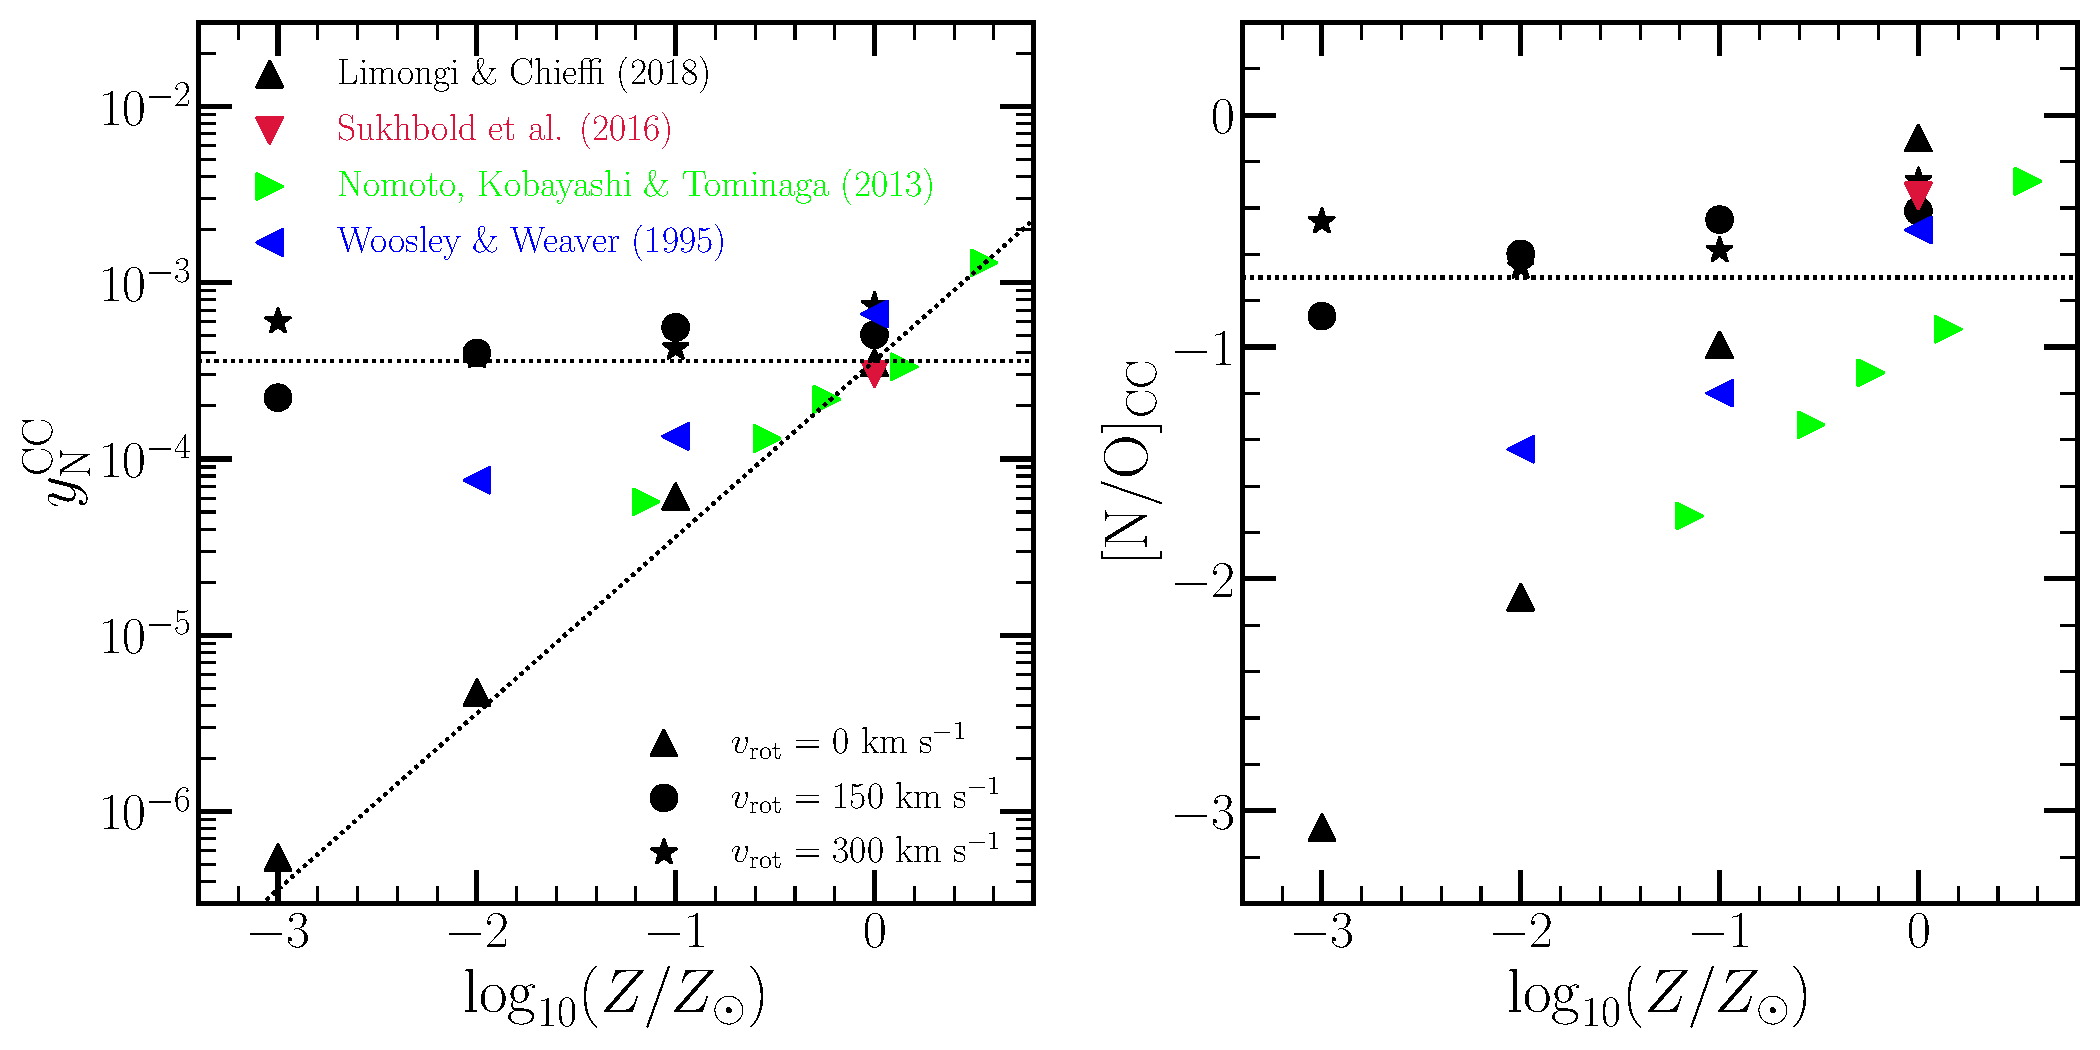
\includegraphics[scale = 0.45]{n_cc_yields.pdf}
\caption{
\textbf{Left}: IMF-averaged CCSN yields of N calculated using~\vice's
\texttt{vice.yields.ccsne.fractional} function with the tables published by
\citet[][blue]{Woosley1995},~\citet[][green]{Nomoto2013},
\citet[][red]{Sukhbold2016}, and~\citet[][black]{Limongi2018}.
All studies report yields for non-rotating progenitors, shown by the triangles;
for visual clarity, the triangles point in a different direction for each study
according to the legend.
\citet{Limongi2018} report additional yields for progenitors with rotational
velocities of 150 (circles) and 300 km/s (stars).
The horizontal dashed line markes~$\ycc{N} = 3.6\times10^{-4}$,
the value of our fiducial CCSN yield of N in our GCE models.
We use the form shown by the slanted line (equation X) in~\S~X in combination
with some of our AGB star yield models discussed in~\S~\ref{sec:yields:agb}.
\textbf{Right}: The~\no~ratio predicted by each of the explosion models in
the left-hand panel, under the same colour-coding and marker scheme.
We mark the position of~$\no = -0.7$ with a black dotted line, the value
roughly suggested by the observations of low-metallicity systems highlighted
in Fig.~\ref{fig:no_oh_observed}.
}
\label{fig:n_cc_yields}
\end{figure*}

We compute theoretically predicted values of~\ycc{N}~using
\vice's~\texttt{vice.yields.ccsne.fractional} function assuming a
\citet{Kroupa2001} IMF; details on how~\vice~handles these calculations can be
found in~\S~4 of~\citet{Griffith2021} and in the~\vice~science 
documentation\footnote{
\url{https://vice-astro.readthedocs.io/en/latest/science_documentation/yields}
}.
In the left panel of Fig.~\ref{fig:n_cc_yields}, we plot the results as a
function of progenitor metallicity as predicted by the~\citet{Woosley1995},
\citet*{Nomoto2013},~\citet{Sukhbold2016}, and~\citet{Limongi2018} tables.
There is good agreement between the various non-rotating models, but only
\citet{Limongi2018} report yields for progenitors with non-zero rotational
velocities; these yields are substantially larger than that of their
non-rotating counterparts.
Most of the N production in CCSN progenitors occurs via the CNO cycle
processing C and O isotopes into~\Nfourteen, and with few C and O seed nuclei
at low~$Z$, production of~\Nfourteen~is difficult.
Rotation-induced mixing, a highly uncertain process~\citep{Zahn1992, Maeder1998,
Lagarde2012}, could transport newly produced C and O into the hydrogen burning
shell of the CCSN progenitor, facilitating~\Nfourteen~production
(\citealp{Frischknecht2016}; see also discussion in~\S~4.2 of
\citealp{Andrews2017}).
For this reason, N yields at low metallicity are quite sensitive to these
assumptions about stellar rotation and internal mixing processes
\citep{Heger2010}, and consequently IMF-averaged yields are highly uncertain.
\par
Based on the definition of the abundance ratio [X/Y], we can compute
the~\no~ratio of CCSN ejecta from the values of~\ycc{N}~and~\ycc{O}~predicted
from a given yield table:
\begin{equation}
\no\subcc = 
\log_{10}\left(\frac{\ycc{N}}{\ycc{O}}\right) -
\log_{10}\left(\frac{Z_{\text{N},\odot}}{Z_{\text{O},\odot}}\right),
\label{eq:no_subcc}
\end{equation}
where~$Z_{\text{X},\odot}$ is the abundance by mass of some element X in the
sun, for which we take~$Z_{\text{N},\odot} = 6.91\times10^{-4}$ and
$Z_{\text{O},\odot} = 5.72\times10^{-3}$ based on the solar photospheric
abundances of~\citet{Asplund2009}.
For each of the published yield tables and rotational velocities in the left
panel of Fig.~\ref{fig:n_cc_yields}, we compute the corresponding values
of~\ycc{O}~using~\vice~and plot the resultant values of~\no\subcc~in the right
panel.
These yield ratios follow similar trends with progenitor metallicity and
rotation as~\ycc{N}~itself, a consequence of the fact that these
studies predict relatively metallicity-independent O yields.
\par
CCSN yields can to some extent be empirically calibrated by ensuring that they
reproduce the~\no~ratios of low metallicity systems.
Since AGB star yields of N are believed to depend on the progenitor's
metallicity (see discussion in~\S~\ref{sec:yields:agb} and references therein),
it's likely that the ``plateau'' in~\no~at low~\oh~reflects the
IMF-averaged CCSN yields of N and O.
Fig.~\ref{fig:no_oh_observed} suggests that~\no\subcc~=~$-0.7$; we highlight
this value in the right panel of Fig.~\ref{fig:n_cc_yields} with a horizontal
black dashed line.
Given this observational result and our adopted value of~$\ycc{O} = 0.015$, we
compute that an empirical N yield of~$\ycc{N} = 3.6\times10^{-4}$ using
equation~\refp{eq:no_subcc}.
We adopt this value as our fiducial CCSN yield of N and highlight it with a
horizontal black dashed line in the left panel of Fig.~\ref{fig:n_cc_yields}.
We discuss the sloped dotted line in that panel in the context of some of our
AGB star yield models in~\S~X.
\par
These empirical values of~\no\subcc~and~\ycc{N}~are in good agreement with
the rotating CCSN models of~\citet{Limongi2018}.
This supports the recent argument by~\citet{Grisoni2021} that rotating massive
stars play an important role in establishing the N abundances observed at low
metallicities in the Milky Way.
Although the~\citet{Sukhbold2016} tables agree nearly perfectly with our
empirical value of~$\ycc{N} = 3.6\times10^{-4}$, they overestimate~\no\subcc~by
$\sim$0.2 dex; this is because they predict a value of~\ycc{O}~lower than our
adopted value of 0.015.
Although most of the supernova models plotted in Fig.~\ref{fig:n_cc_yields}
slightly overestimate our empirical value of~\no\subcc~=~$-0.7$, they still
fall short of solar.
This implies the need for an additional enrichment, which is expected because
it is well understood that N is also produced in considerable amounts by
AGB stars~\citep{Johnson2019}.


\subsection{Asymptotic Giant Branch Stars}
\label{sec:yields:agb}

Similar to our SN yields (see discussion in~\S~\ref{sec:yields:ccsne}), our
AGB star yields are fractional net yields in that they quantify only the newly
produced mass of an element X in units of the progenitor star's zero-age main
sequence (ZAMS) mass.
For a yield~$\yagb{X}(M_\star, Z_\star)$, the mass yield is then
given by~$M_\star \yagb{X}(M_\star, Z_\star)$.
AGB star enrichment proceeds as it does in~\citet{Johnson2020} under the caveat
that the yield is placed in the~$\delta\rgal = 100$ pc ring that a stellar
population is in at a given time.
In short,~\vice~implements an algorithm which computes the mass in dying stars
from each stellar population, and the ZAMS mass required to compute the
fractional yield comes from a mass-lifetime relationship; for the latter, we
adopt the parabola in~$\log\tau - \log m$ space from~\citet{Larson1974} (see
discussion of the mass-lifetime relationship in~\vice~in Appendix
\ref{sec:vice}).

\begin{figure*}
\centering
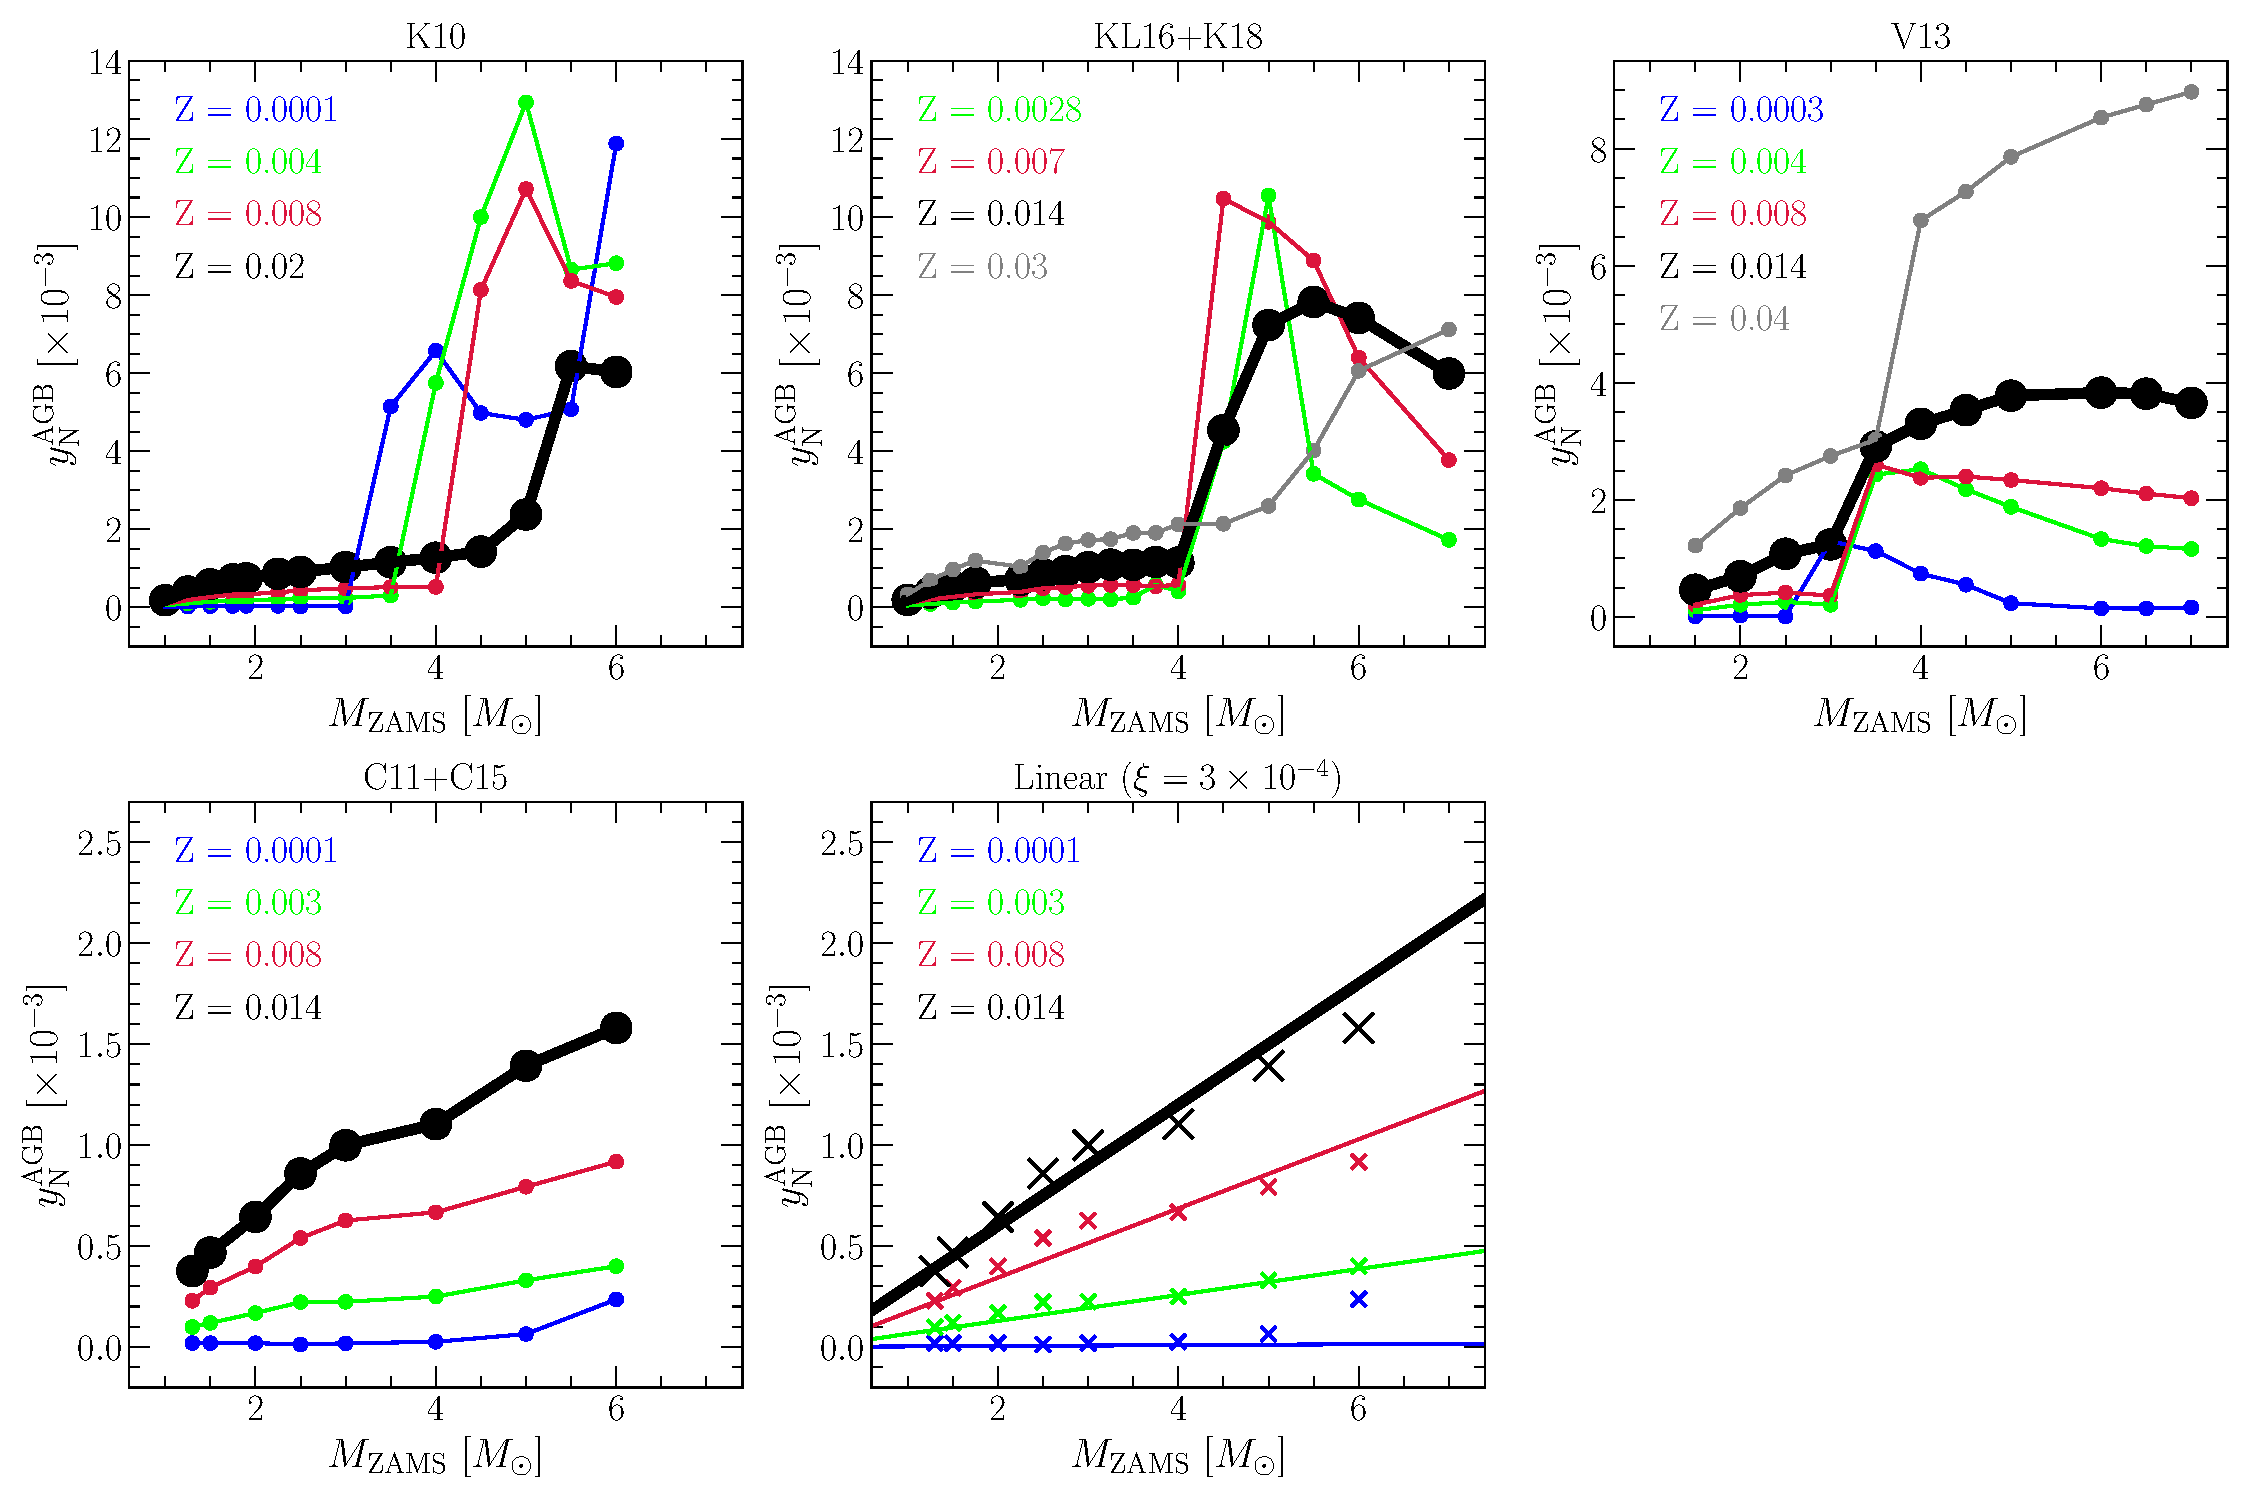
\includegraphics[scale = 0.32]{agb_yield_models.pdf}
\caption{
The fractioanl yields of N from AGB stars~\yagb{N}~as a function of progenitor
ZAMS mass and birth metallicity~$Z$ as reported by
\citet[][upper left]{Karakas2010},~\citet{Karakas2016} and
\citet[][upper middle]{Karakas2018},~\citet[][upper right]{Ventura2013,
Ventura2014, Ventura2018, Ventura2020}, and~\citet[][lower right]{Cristallo2011,
Cristallo2015}.
For~\citet{Ventura2013, Ventura2014, Ventura2018, Ventura2020} and
\citet{Cristallo2011, Cristallo2015}, we show the yields only for a selection
of metallicities available from their provided tables.
We highlight yields at solar metallicity ($Z = 0.02$ for~\citealp{Karakas2010},
$Z = 0.014$ otherwise) with bold black lines.
In the lower right panel, we show the yields predicted by our linear model
(coloured lines, see discussion in~\S~\ref{sec:yields:agb}) in comparison to
the~\citet[][coloured X's]{Cristallo2011, Cristallo2015} predictions.
}
\label{fig:agb_yield_models}
\end{figure*}

Here we make use of four previously published tables of AGB star yields
calculated from stellar evolution models, each of which are sampled on a grid
of progenitor masses and metallicities.
To approximate~\yagb{X}~as a smooth function of~$M_\star$ and
$Z_\star$,~\vice~interpolates bi-linearly between grid elements - once in
mass and once in metallicity - and linearly extrapolates above or below in
either quantity as necessary.
By comparing the predicted N abundances of the~\citet{Johnson2021} chemical
evolution model for the Milky Way to the latest observational data, we can
constrain how accurately these ``off-the-shelf'' yield models characterize
how and where N is produced:
\begin{itemize}
	\item[\textbf{1.}] \citet[][hereafter~\karakasten]{Karakas2010}\footnote{
		We clarify that our abbreviations of these papers (i.e.~\karakasten,
		\karakas,~\ventura, and~\cristallo) refer specifically to their yields
		of N as we adopt them in our model.
		We cite the full names of these papers when referring to their more
		general results.
	} published yields for~$Z = 0.0001$, 0.004, 0.008, and 0.02 progenitors.
	We plot these yields in the upper left panel of 
	Fig.~\ref{fig:agb_yield_models}.

	\item[\textbf{2.}] \citet{Karakas2016} and~\citet{Karakas2018} published
	yields for~$Z = 0.0028$, 0.007, 0.014, and 0.03 progenitors; we hereafter
	refer to these yields as the~\karakas~model.
	We plot a subset of these yields in the upper middle panel of
	Fig.~\ref{fig:agb_yield_models}.

	\item[\textbf{3.}] We combine the yields for~$Z = 0.0003$ and 0.008
	progenitors from~\citet{Ventura2013} with those at~$Z = 0.004$ from
	\citet{Ventura2014}, at~$Z = 0.014$ from~\citet{Ventura2018}, and at
	$Z = 0.04$ from~\citet{Ventura2020} into a single table of yields.
	In this set, we also include a set of un-published yields at~$Z = 0.001$
	and 0.002 computed with similar stellar models (provided by P. Ventura,
	private communication).
	We hereafter refer to this yield set as the~\ventura~model, and we
	illustrate a subsample of these yields in the upper right panel of
	Fig.~\ref{fig:agb_yield_models}.

	\item[\textbf{4.}] \citet{Cristallo2011, Cristallo2015} published yields
	for~$Z = 0.0001$, 0.0003, 0.001, 0.002, 0.003, 0.006, 0.008, 0.01, 0.014,
	and 0.02 progenitors; we hereafter refer to these yields as
	the~\cristallo~model.
	This is the default set of yields in~\vice.
	It is also the software's most comprehensive set of previously published
	AGB star yields in that it includes tables for all elements built into the
	code and is sampled at the most metallicities.
	We illustrate a subsample of these yields in the lower left panel of
	Fig.~\ref{fig:agb_yield_models}.
\end{itemize}
\vice~also allows users to construct their own functions of progenitor mass
and metallicity to describe the AGB star yield.
Motivated by the roughly linear of the~\cristallo~yields and their general
success in our fiducial model once renormalized by a constant factor (see
discussion in~\S~\ref{sec:results}), we construct a model in which the yield
is linearly proportional to both progenitor ZAMS mass and metallicity:
\begin{equation}
\yagb{N} = \xi \left(\frac{M}{M_\odot}\right) \left(\frac{Z}{Z_\odot}\right)
\end{equation}
We illustrate this model in the lower middle panel of Fig.
\ref{fig:agb_yield_models} for~$\xi = 3\times10^{-4}$ in comparison to
the~\cristallo~yields shown by the coloured X's.
\par
Despite reporting values of the same physical quantities, the N yields
reported by each of these studies show substantial differences between one
another.
Unfortunately, ascertaining the origins of these differences is difficult
because each study employs different assumptions for opacity, mass loss,
nuclear reaction networks, and convection and convective boundaries within
stars, all of which have a significant impact on stellar evolution and thus
the predicted yields (see discussion in, e.g.,~\S~5 of~\citealp{Karakas2016}).
However, the differences can largely be understood by considering two important
phenomena known to occur within AGB stars: third dredge-up (TDU) and hot bottom
burning (HBB).
Collapsing the information into these two processes is helpful because their
differences arise as a consequence of the different input physics between the
stellar evolution models.
\par
TDU refers to the repeated penetrations of the convected envelope into the
hydrogen-depleted core during the thermal pulses associated with AGB star
evolution.
This process doesn't affect N abundances much because at this evolutionary
phase, the core is mostly composed of C and O.
However, the~\Cthirteen($\alpha$, n)\Osixteen~reaction can occur at substantial
rates when the core material is mixed with the He-rich shell during each TDU
episode.
This reaction is the main source of free neutrons in low mass AGB stars, and as
a consequence, each replenishment of C does indirectly contribute to raising
an AGB star's overall yield.
HBB refers to proton capture reactions at the base of the convective envelope.
This activates the CNO cycle, producing large amounts of~\Nfourteen~at the
expense of C and O isotopes.
HBB requires a higher mass AGB star progenitor ($M_\text{ZAMS} = 4 - 5~M_\odot$
at~$Z_\odot$ according to~\citealt{Karakas2010}) than TDU
($M_\text{ZAMS} = 2 - 2.5~M_\odot$ at~$Z_\odot$ according to
\citealt{Karakas2010}), but the minimum mass for both decreases at lower
metallicities.
\par
The most efficient N production occurs when both TDU and HBB are active within
an AGB star, because each replenishment of C and O isotopes by TDU adds new
seed nuclei for the CNO cycle when HBB is active.
This is the reason for the substantial N production above~$\sim4~M_\odot$ in
the~\karakasten~and~\karakas~models; in both yield sets, every star that
experiences HBB also experiences TDU (see Table 1 in both~\citealt{Karakas2010}
and~\citealt{Karakas2014}, which describes the stellar evolution models from
which the~\karakas~yields are computed).
Both TDU and HBB are more efficient at low metallicity (see discussion in
\citealt{Ventura2013}).
In the case of TDU, each penetration into the core by the convective envelope
is deeper due to the lower opacity.
For HBB, the base of the convective is hotter at low~$Z$, and the rate of CNO
cycle reactions is an extremely strong function of temperature.
This interaction between TDU and HBB is also the reason for the increase in N
yields in the~\ventura~tables near~$\sim3~M_\odot$.
Unlike the~\karakasten~and~\karakas~models, their stars experience both TDU and
HBB only in this narrow mass range.
\par
Of all of these yields taken from the literature, the~\cristallo~sample shows
the smoothest dependence on progenitor mass and metallicity.
Unfortunately, ascertaining the exact cause of this difference between other
yields explored here is difficult even when collapsing the information into
TDU and HBB.
Relative to the~\karakas~yields (see discussion in~\S~5 of
\citealt{Karakas2016}), the~\cristallo~models have more mass loss, a~$\sim$10\%
faster triple-$\alpha$ reaction rate, fewer thermal pulses overall, and weaker
HBB due to a lower temperature at the base of the convective envelope.
Though their agreement is good below~$\sim3~M_\odot$, the fact that HBB is
weaker and there are fewer TDU episodes does however lend a qualitative
explanation into why the~\cristallo~yields are so much smaller than
the~\karakasten~and~\karakas~yields at higher masses.
\par
Although both the~\karakasten~and~\karakas~yield models both show a substantial
increase in N yields above~$\sim4~M_\odot$, there are some notable differences
between the two.
In particular, the yields at solar metallicity are somewhat higher in the
newer version.
Some of this can be attributed to the now-lowered solar metallicity\footnote{
Changes in the adopted solar metallicity trace back to the canonical value of
$\sim$2\%~\citep*{Anders1989, Grevesse1993, Grevesse1998} later being revised
to~$\sim$1.4\% (\citealp*{Lodders2003, Asplund2005, Lodders2009};
\citealp{Asplund2009};~\citealp*{Asplund2021}).
} ($Z = 0.014$ in~\karakas~compared to~$Z = 0.02$ in~\karakasten) and the
effect that has on TDU and HBB, but this does not account for all of the
differences.
Furthermore, the yields at sub-solar metallicities decreased slightly
from~\karakasten~to~\karakas, particularly for the highest mass AGB stars.
These differences can be understood by slight variations in the input physics
(A. Karakas, private communication).
Based on updated opacity tables, the~\karakas~models are slightly hotter and
more compact; consequently, they experience hotter HBB and deeper TDU.
Experiencing more thermal pulses overall and consequently a longer AGB lifetime,
the~\karakas~stars have more time for HBB to convert~\Ctwelve~into~\Nfourteen.
At lower metallicity,~\karakas~use low-temperature opacity tables based on
\citet{Marigo2002} that more closely follow the surface composition of the
star.
These opacities are higher, making the stars larger and increasing the
mass-loss rate relative to~\karakasten.
The~$Z = 0.0028$ model from~\citet{Karakas2018} uses the~\citet{Bloecker1995}
mass-loss prescription as opposed to that of~\citet{Vassiliadis1993} as in
both~\citet{Karakas2010}~and~\citet{Karakas2016}.
This choice results in fewer thermal pulses and a shorter AGB lifetime.
Each of these effects at low metallicity act to decrease the overall yield
of~\Nfourteen.
\par
In the interest of consistency, when we adopt a particular AGB star yield model
for N, we also adopt the corresponding table within~\vice~for O and Fe when
possible.\footnote{
	In the case of~\citet{Ventura2013, Ventura2014, Ventura2018, Ventura2020},
	AGB star yields of Fe are not available.
	In the case of our linear model which applies only to N, we assume 
	the~\vice~default of the~\citet{Cristallo2011, Cristallo2015} yields for
	both O and Fe.
}

\subsection{IMF-Averaged AGB Star Yields: Metallicity and Time Dependence}
\label{sec:yields:imf_agb}

\begin{figure*}
\centering
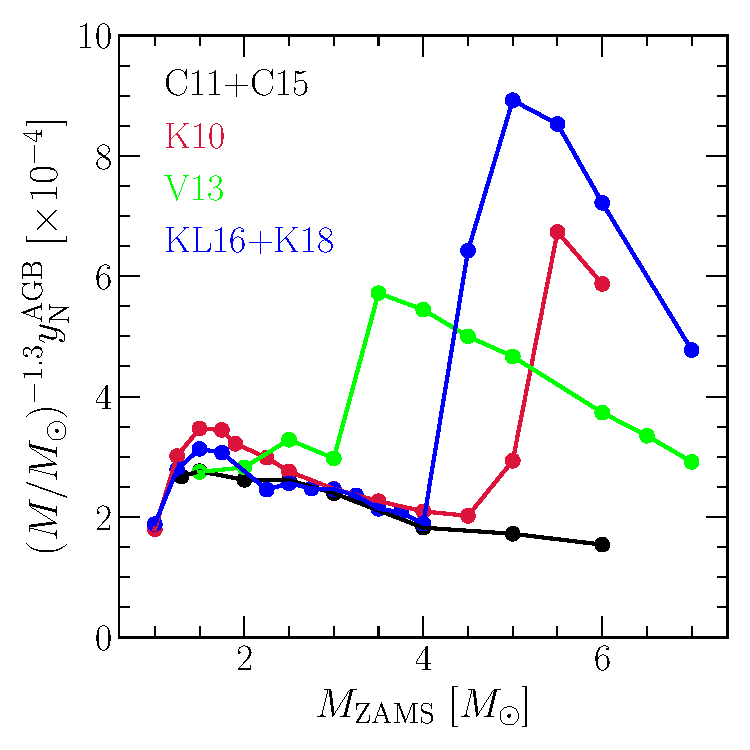
\includegraphics[scale = 0.32]{agb_yield_models_imfweighted.pdf}
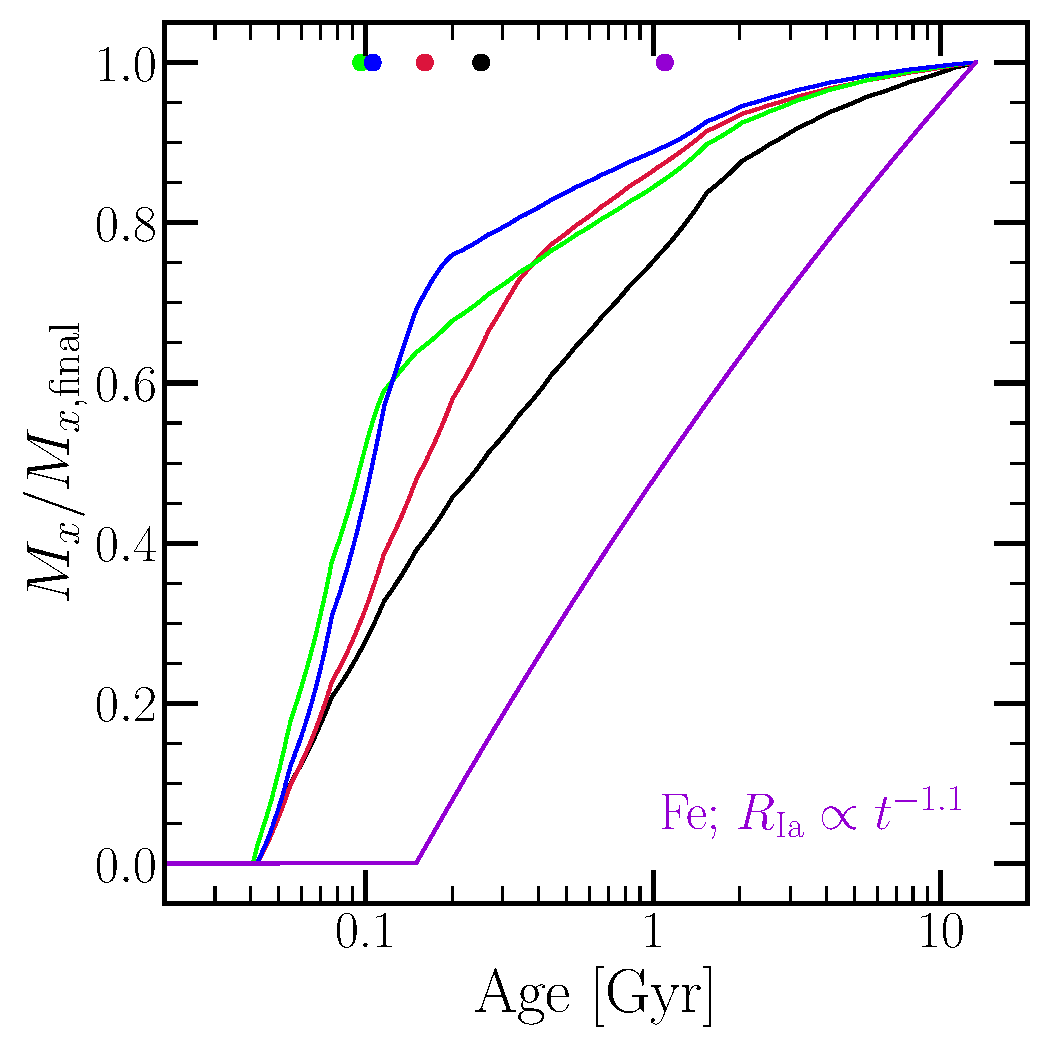
\includegraphics[scale = 0.32]{ssp_production_modelcomp.pdf}
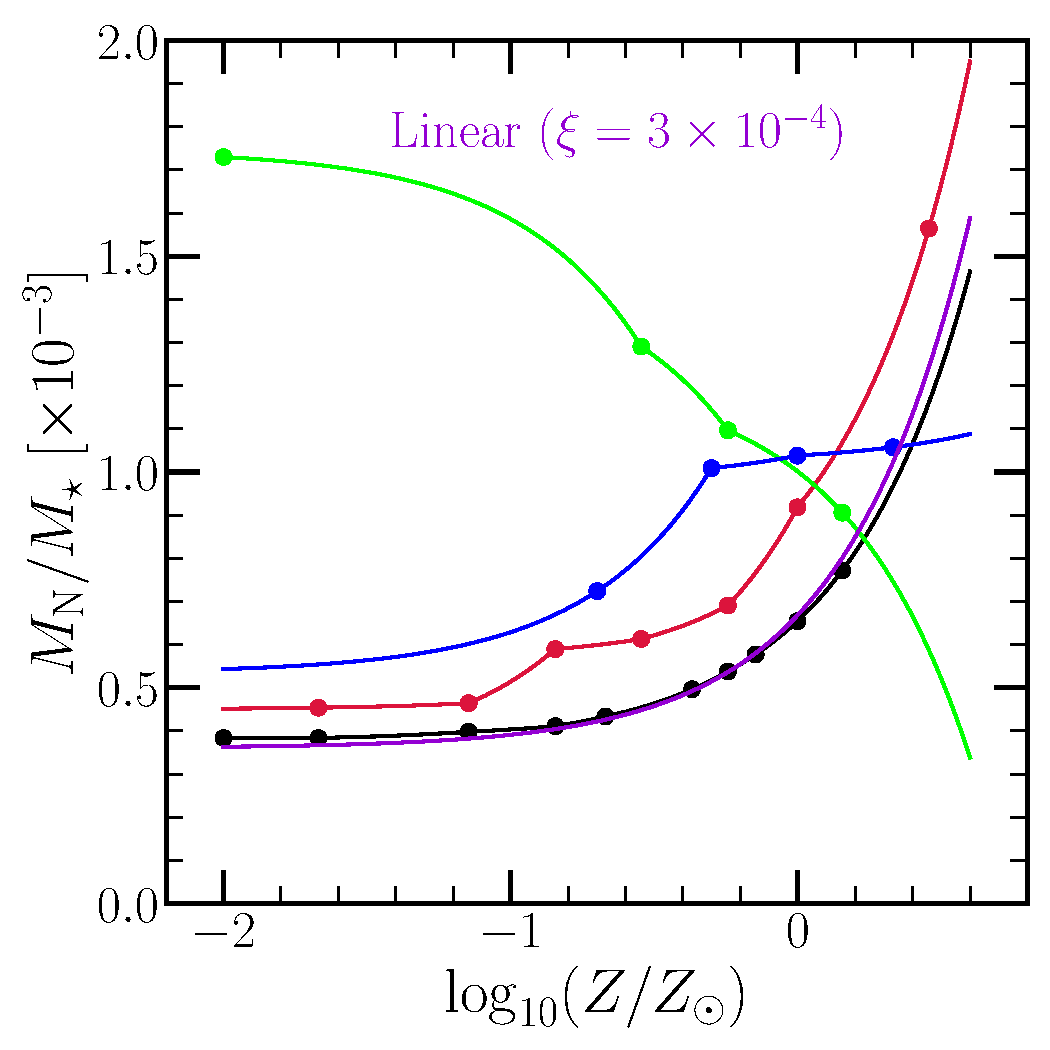
\includegraphics[scale = 0.32]{ssp_production_metdep.pdf}
\caption{
\textbf{Left}: The IMF-weighted mass yield of N from AGB stars as a function of
progenitor ZAMS mass at solar metallicity ($Z = 0.02$ in~\karakasten,
$Z = 0.014$ otherwise).
\textbf{Middle}: The net mass of N produced by AGB stars from a single stellar
population for each of our yield models at solar metallicity.
The purple line denotes the same for Fe assuming our~$t^{-1.1}$ DTD as in the
\citet{Johnson2021} chemical evolution model.
All values are normalized to the total mass produced at an age of 13.2 Gyr.
Points at the top of the panel denote the ages at which 50\% of the total mass
yield has been produced.
\textbf{Right}: The total amount of N produced by a 13.2 Gyr old stellar
population as a function of metallicity for each of our yield models normalized
by the stellar population's initial mass.
Points mark metallicities at which the published tables report yields.
}
\label{fig:ssp}
\end{figure*}

To more directly compare the~\karakasten,~\karakas,~\ventura,
and~\cristallo~AGB star yield models of N to one another, we plot IMF-weighted
yields from each of them at solar metallicity ($Z = 0.02$ for~\karakasten,
$Z = 0.02$ otherwise) in the left hand panel of Fig.~\ref{fig:ssp}.
As mentioned in~\S~\ref{sec:yields:agb}, the AGB star yield of N~\yagb{N}~as we
have parameterized it is in units of the progenitor star's ZAMS mass, and
consequently the~\textit{mass yield} of N is given by~$M_\star \yagb{N}$.
With an additional weight of~$M_\star^{-2.3}$ from the IMF in this mass range
\citep[e.g.][]{Kroupa2001}, we therefore multiply the values of~\yagb{N}~by
$(M_\star / M_\odot)^{-1.3}$ to quantify the total mass yield of N taking into
account the intrinsic mass distribution of stars.
Even with the additional weight of~$M_\star^{-1.3}$, the~\cristallo~yields are
relatively mass-independent.
For other studies, the contributions from higher mass AGB stars is yet more
pronounced due to the effects of TDU and HBB discussed
in~\S~\ref{sec:yields:agb}.
\par
In the middle panel of Fig.~\ref{fig:ssp}, we plot the AGB star production of
N from a single stellar population as a function of its age.
For this we use~\vice's~\texttt{vice.single\_stellar\_population} function
which computes the mass yield of a given element as a function of age from a
star cluster of known metallicity.
For the sake of this calculation, we set all CCSN yields of N to zero in order
to highlight the AGB star contribution.
We show the results of this procedure for solar metallicity only (again
$Z = 0.02$ for~\karakasten,~$Z = 0.014$ otherwise), and we normalize all values
to the total mass produced at~$T = 13.2$ Gyr.
\par
Under the~\cristallo~yields, it takes~$\sim$250 Myr for a single stellar
population to produce~$\sim$50\% of its N from AGB stars, as noted by the
coloured points at the top of the panel.
This is a rather short characteristic delay time considering that these yields
are relatively mass-independent when weighted by the IMF, suggesting
instead that most of the N yield under this model is actually coming from
higher mass ($\gtrsim 2~M_\odot$) AGB stars.
This traces back to the steep nature of the stellar mass-lifetime relation
\citep[e.g.][]{Larson1974, Maeder1989, Padovani1993}.
Even though the IMF-weighted yields suggest roughly equal contributions per
small interval in mass~$dM_\star$, this quantifies the contributions per small
interval in age~$d\tau$.
As a stellar population ages, the enrichment rates will inevitably slow down
considerably as the mass range~$dM_\star$ gets progressively narrower as~$\tau$
increases.
As expected due to their larger IMF-weighted contributions to N from high mass
AGB stars, our other yield models predict even shorter characteristic delay
times.
\par
For comparison, we plot the enrichment of Fe by our~$t^{-1.1}$ power-law DTD,
also with the CCSN yield set to zero to highlight the SN Ia contribution.
The characteristic delay time for Fe production is longer than that of N by
nearly an order of magnitude - exactly how much depending on which AGB star
yield model is selected.
As noted in~\citet{Johnson2021}, a delay-time of~$\sim$1 Gyr is exactly as
expected for a~$\sim t^{-1}$ DTD because half of the SNe Ia occur between
100 Myr and 1 Gyr and and the other half between 1 Gyr and 10 Gyr.
\par
In the right panel of Fig.~\ref{fig:ssp}, we plot the total amount of N
produced by a 13.2 Gyr old single stellar population as a function of its
metallicity according to all of our AGB star yield models, including the linear
model (see discussion in~\S~\ref{sec:yields:agb}).
For this calculation, we retain our CCSN yield of N (see discussion
in~\S~\ref{sec:yields:ccsne}):~$\ycc{N} = 3.6\times10^{-4}$.
In general, there is good qualitative agreement between the~\cristallo~and
the~\ventura~models, the only major difference being the normalization.
The predictions with the linear model with~$\xi = 3\times10^{-4}$ are nearly
identical to the~\cristallo~model, though this is unsurprising given their
similarity in Fig.~\ref{fig:agb_yield_models}.
The value at which these N yields flatten off at low~$Z$ is reflective of our
adopted value of~\ycc{N}.
Up to~$\log_{10}(Z / Z_\odot) \approx -0.2$, the~\karakas~yields predict a
similar trend as~\cristallo~and~\ventura, also with a difference in
normalization, but at solar and super-solar metallicities they predict much
more metallicity-independent N yields than others.
The~\karakasten~yields, on the other hand, do not agree with any of the other
models, instead predicting N yields to~\textit{decrease} monotonically with
increasing~$Z$.
These differences between the~\karakasten~and~\karakas~models traces back to
differences regarding the opacity and mass loss prescriptions between these
two models (see discussion in~\S~\ref{sec:yields:agb}).
We demonstrate in~\S~\ref{sec:results:yields} that N yields which scale roughly
linearly with metallicity as in the~\cristallo~and~\ventura~models are required
in order to reproduce the~\ohno~relation as observed.
The normalization, however, depends on the SN yields.

\end{document}

